%%%%%%%%%%%%%%%%%%%%%%%%%%%%%%%%%%%%%%%%%
% The Legrand Orange Book
% LaTeX Template
% Version 2.0 (9/2/15)
% This template has been downloaded from:
% http://www.LaTeXTemplates.com
% Mathias Legrand (legrand.mathias@gmail.com) with modifications by:
% Vel (vel@latextemplates.com)
%
% License:
% CC BY-NC-SA 3.0 (http://creativecommons.org/licenses/by-nc-sa/3.0/)
%
% Important note:
% Chapter heading images should have a 2:1 width:height ratio,
% e.g. 920px width and 460px height.
%%%%%%%%%%%%%%%%%%%%%%%%%%%%%%%%%%%%%%%%%
%  Adaptado por Prof. Ausberto Castro Vera,
%  2013-2022
%%%%%%%%%%%%%%%%%%%%%%%%%%%%%%%%%%%%%%%%%
%  Escrito por Eric Hoffmann Fernandes Braga
%  2024
%%%%%%%%%%%%%%%%%%%%%%%%%%%%%%%%%%%%%%%%%
%----------------------------------------------------------------------------------------
%	PACKAGES AND OTHER DOCUMENT CONFIGURATIONS
%----------------------------------------------------------------------------------------

\documentclass[11pt,fleqn]{book} % Default font size and left-justified equations

%----------------------------------------------------------------------------------------

%%%%%%%%%%%%%%%%%%%%%%%%%%%%%%%%%%%%%%%%%
% The Legrand Orange Book 
% Structural Definitions File
% Version 2.0 (9/2/15)
%
% Original author:
% Mathias Legrand (legrand.mathias@gmail.com) with modifications by:
% Vel (vel@latextemplates.com)
%
% This file has been downloaded from:
% http://www.LaTeXTemplates.com
%
% License: 
% CC BY-NC-SA 3.0 (http://creativecommons.org/licenses/by-nc-sa/3.0/)
%
%%%%%%%%%%%%%%%%%%%%%%%%%%%%%%%%%%%%%%%%%%

%----------------------------------------------------------------------------------------
%	VARIOUS REQUIRED PACKAGES AND CONFIGURATIONS
%----------------------------------------------------------------------------------------

\usepackage[top=3cm,bottom=3cm,left=3cm,right=3cm,headsep=10pt,a4paper]{geometry} % Page margins

\usepackage{graphicx} % Required for including pictures
\graphicspath{{Pictures/}} % Specifies the directory where pictures are stored

\usepackage{lipsum} % Inserts dummy text
\usepackage{here}   %
\usepackage{tikz} % Required for drawing custom shapes

\usepackage[brazil]{babel} % Brazilian Portuguese language/hyphenation

\usepackage{enumitem} % Customize lists
\setlist{nolistsep} % Reduce spacing between bullet points and numbered lists

\usepackage{booktabs} % Required for nicer horizontal rules in tables

% \usepackage[table,xcdraw]{xcolor}
\usepackage{xcolor}
\definecolor{ocre}{RGB}{243,102,25} % Define the orange color used for highlighting throughout the book

\usepackage{bibentry}
%----------------------------------------------------------------------------------------
%	FONTS
%----------------------------------------------------------------------------------------

\usepackage{avant} % Use the Avantgarde font for headings
%\usepackage{times} % Use the Times font for headings
\usepackage{mathptmx} % Use the Adobe Times Roman as the default text font together with math symbols from the Sym­bol, Chancery and Com­puter Modern fonts

\usepackage{microtype} % Slightly tweak font spacing for aesthetics
\usepackage[utf8]{inputenc} % Required for including letters with accents
\usepackage[T1]{fontenc} % Use 8-bit encoding that has 256 glyphs

%----------------------------------------------------------------------------------------
%	CODE BLOCKS AND COLORS
%----------------------------------------------------------------------------------------

\usepackage[many]{tcolorbox}
\usepackage{color}
\usepackage{listings}
\definecolor{GrayCodeBlock}{RGB}{241,241,241}
\definecolor{BlackText}{RGB}{110,107,94}
\definecolor{RedTypename}{RGB}{182,86,17}
\definecolor{GreenString}{RGB}{96,172,57}
\definecolor{PurpleKeyword}{RGB}{184,84,212}
\definecolor{GrayComment}{RGB}{170,170,170}
\definecolor{GoldDocumentation}{RGB}{180,165,45}
\lstdefinelanguage{rust}
{
    columns=fullflexible,
    keepspaces=true,
    frame=single,
    framesep=0pt,
    framerule=0pt,
    framexleftmargin=4pt,
    framexrightmargin=4pt,
    framextopmargin=5pt,
    framexbottommargin=3pt,
    xleftmargin=4pt,
    xrightmargin=4pt,
    backgroundcolor=\color{GrayCodeBlock},
    basicstyle=\ttfamily\color{BlackText},
    keywords={
        true,false,
        unsafe,async,await,move,
        use,pub,crate,super,self,mod,
        struct,enum,fn,const,static,let,mut,ref,type,impl,dyn,trait,where,as,
        break,continue,if,else,while,for,loop,match,return,yield,in
    },
    keywordstyle=\color{PurpleKeyword},
    ndkeywords={
        bool,u8,u16,u32,u64,u128,i8,i16,i32,i64,i128,isize,usize,char,str,
        Self,Option,Some,None,Result,Ok,Err,String,Box,Vec,Rc,Arc,Cell,RefCell,HashMap,BTreeMap,
        macro_rules
    },
    ndkeywordstyle=\color{RedTypename},
    comment=[l][\color{GrayComment}\slshape]{//},
    morecomment=[s][\color{GrayComment}\slshape]{/*}{*/},
    morecomment=[l][\color{GoldDocumentation}\slshape]{///},
    morecomment=[s][\color{GoldDocumentation}\slshape]{/*!}{*/},
    morecomment=[l][\color{GoldDocumentation}\slshape]{//!},
    morecomment=[s][\color{RedTypename}]{\#![}{]},
    morecomment=[s][\color{RedTypename}]{\#[}{]},
    stringstyle=\color{GreenString},
    string=[b]"
}
%----------------------------------------------------------------------------------------
%       TERMINAL EMULATION
%----------------------------------------------------------------------------------------
\lstdefinelanguage{bash}
{
    columns=fullflexible,
    keepspaces=true,
    frame=single,
    framesep=0pt,
    framerule=0pt,
    framexleftmargin=4pt,
    framexrightmargin=4pt,
    framextopmargin=5pt,
    framexbottommargin=3pt,
    xleftmargin=4pt,
    xrightmargin=4pt,
    backgroundcolor=\color{GrayCodeBlock},
    basicstyle=\ttfamily\color{BlackText},
}

%----------------------------------------------------------------------------------------
%	BIBLIOGRAPHY AND INDEX
%----------------------------------------------------------------------------------------
\usepackage{hyperref}



\sloppy




%\usepackage[style=alphabetic, citestyle=numeric, sorting=nyt, sortcites=true,
%            autopunct=true, babel=hyphen, hyperref=true, abbreviate=false,
%            backref=true, backend=biber]{biblatex}
%\addbibresource{racketbib.bib} % BibTeX bibliography file
%\defbibheading{bibempty}{}

\usepackage{calc} % For simpler calculation - used for spacing the index letter headings correctly
\usepackage{makeidx} % Required to make an index
\makeindex % Tells LaTeX to create the files required for indexing

%----------------------------------------------------------------------------------------
%	MAIN TABLE OF CONTENTS
%----------------------------------------------------------------------------------------

\usepackage{titletoc} % Required for manipulating the table of contents

\contentsmargin{0cm} % Removes the default margin

% Part text styling
\titlecontents{part}[0cm]
{\addvspace{20pt}\centering\large\bfseries}
{}
{}
{}

% Chapter text styling
\titlecontents{chapter}[1.25cm] % Indentation
{\addvspace{12pt}\large\sffamily\bfseries} % Spacing and font options for chapters
{\color{ocre!60}\contentslabel[\Large\thecontentslabel]{1.25cm}\color{ocre}} % Chapter number
{\color{ocre}}
{\color{ocre!60}\normalsize\;\titlerule*[.5pc]{.}\;\thecontentspage} % Page number

% Section text styling
\titlecontents{section}[1.25cm] % Indentation
{\addvspace{3pt}\sffamily\bfseries} % Spacing and font options for sections
{\contentslabel[\thecontentslabel]{1.25cm}} % Section number
{}
{\hfill\color{black}\thecontentspage} % Page number
[]

% Subsection text styling
\titlecontents{subsection}[1.25cm] % Indentation
{\addvspace{1pt}\sffamily\small} % Spacing and font options for subsections
{\contentslabel[\thecontentslabel]{1.25cm}} % Subsection number
{}
{\ \titlerule*[.5pc]{.}\;\thecontentspage} % Page number
[]

% List of figures
\titlecontents{figure}[0em]
{\addvspace{-5pt}\sffamily}
{\thecontentslabel\hspace*{1em}}
{}
{\ \titlerule*[.5pc]{.}\;\thecontentspage}
[]

% List of tables
\titlecontents{table}[0em]
{\addvspace{-5pt}\sffamily}
{\thecontentslabel\hspace*{1em}}
{}
{\ \titlerule*[.5pc]{.}\;\thecontentspage}
[]

%----------------------------------------------------------------------------------------
%	MINI TABLE OF CONTENTS IN PART HEADS
%----------------------------------------------------------------------------------------

% Chapter text styling
\titlecontents{lchapter}[0em] % Indenting
{\addvspace{15pt}\large\sffamily\bfseries} % Spacing and font options for chapters
{\color{ocre}\contentslabel[\Large\thecontentslabel]{1.25cm}\color{ocre}} % Chapter number
{}
{\color{ocre}\normalsize\sffamily\bfseries\;\titlerule*[.5pc]{.}\;\thecontentspage} % Page number

% Section text styling
\titlecontents{lsection}[0em] % Indenting
{\sffamily\small} % Spacing and font options for sections
{\contentslabel[\thecontentslabel]{1.25cm}} % Section number
{}
{}

% Subsection text styling
\titlecontents{lsubsection}[.5em] % Indentation
{\normalfont\footnotesize\sffamily} % Font settings
{}
{}
{}

%----------------------------------------------------------------------------------------
%	PAGE HEADERS
%----------------------------------------------------------------------------------------

\usepackage{fancyhdr} % Required for header and footer configuration

\pagestyle{fancy}
\renewcommand{\chaptermark}[1]{\markboth{\sffamily\normalsize\bfseries\chaptername\ \thechapter.\ #1}{}} % Chapter text font settings
\renewcommand{\sectionmark}[1]{\markright{\sffamily\normalsize\thesection\hspace{5pt}#1}{}} % Section text font settings
\fancyhf{} \fancyhead[LE,RO]{\sffamily\normalsize\thepage} % Font setting for the page number in the header
\fancyhead[LO]{\rightmark} % Print the nearest section name on the left side of odd pages
\fancyhead[RE]{\leftmark} % Print the current chapter name on the right side of even pages
\renewcommand{\headrulewidth}{0.5pt} % Width of the rule under the header
\addtolength{\headheight}{2.5pt} % Increase the spacing around the header slightly
\renewcommand{\footrulewidth}{0pt} % Removes the rule in the footer
\fancypagestyle{plain}{\fancyhead{}\renewcommand{\headrulewidth}{0pt}} % Style for when a plain pagestyle is specified

% Removes the header from odd empty pages at the end of chapters
\makeatletter
\renewcommand{\cleardoublepage}{
\clearpage\ifodd\c@page\else
\hbox{}
\vspace*{\fill}
\thispagestyle{empty}
\newpage
\fi}

%----------------------------------------------------------------------------------------
%	THEOREM STYLES
%----------------------------------------------------------------------------------------

\usepackage{amsmath,amsfonts,amssymb,amsthm} % For math equations, theorems, symbols, etc

\newcommand{\intoo}[2]{\mathopen{]}#1\,;#2\mathclose{[}}
\newcommand{\ud}{\mathop{\mathrm{{}d}}\mathopen{}}
\newcommand{\intff}[2]{\mathopen{[}#1\,;#2\mathclose{]}}
\newtheorem{notation}{Notation}[chapter]

% Boxed/framed environments
\newtheoremstyle{ocrenumbox}% % Theorem style name
{0pt}% Space above
{0pt}% Space below
{\normalfont}% % Body font
{}% Indent amount
{\small\bf\sffamily\color{ocre}}% % Theorem head font
{\;}% Punctuation after theorem head
{0.25em}% Space after theorem head
{\small\sffamily\color{ocre}\thmname{#1}\nobreakspace\thmnumber{\@ifnotempty{#1}{}\@upn{#2}}% Theorem text (e.g. Theorem 2.1)
\thmnote{\nobreakspace\the\thm@notefont\sffamily\bfseries\color{black}---\nobreakspace#3.}} % Optional theorem note
\renewcommand{\qedsymbol}{$\blacksquare$}% Optional qed square

\newtheoremstyle{blacknumex}% Theorem style name
{5pt}% Space above
{5pt}% Space below
{\normalfont}% Body font
{} % Indent amount
{\small\bf\sffamily}% Theorem head font
{\;}% Punctuation after theorem head
{0.25em}% Space after theorem head
{\small\sffamily{\tiny\ensuremath{\blacksquare}}\nobreakspace\thmname{#1}\nobreakspace\thmnumber{\@ifnotempty{#1}{}\@upn{#2}}% Theorem text (e.g. Theorem 2.1)
\thmnote{\nobreakspace\the\thm@notefont\sffamily\bfseries---\nobreakspace#3.}}% Optional theorem note

\newtheoremstyle{blacknumbox} % Theorem style name
{0pt}% Space above
{0pt}% Space below
{\normalfont}% Body font
{}% Indent amount
{\small\bf\sffamily}% Theorem head font
{\;}% Punctuation after theorem head
{0.25em}% Space after theorem head
{\small\sffamily\thmname{#1}\nobreakspace\thmnumber{\@ifnotempty{#1}{}\@upn{#2}}% Theorem text (e.g. Theorem 2.1)
\thmnote{\nobreakspace\the\thm@notefont\sffamily\bfseries---\nobreakspace#3.}}% Optional theorem note

% Non-boxed/non-framed environments
\newtheoremstyle{ocrenum}% % Theorem style name
{5pt}% Space above
{5pt}% Space below
{\normalfont}% % Body font
{}% Indent amount
{\small\bf\sffamily\color{ocre}}% % Theorem head font
{\;}% Punctuation after theorem head
{0.25em}% Space after theorem head
{\small\sffamily\color{ocre}\thmname{#1}\nobreakspace\thmnumber{\@ifnotempty{#1}{}\@upn{#2}}% Theorem text (e.g. Theorem 2.1)
\thmnote{\nobreakspace\the\thm@notefont\sffamily\bfseries\color{black}---\nobreakspace#3.}} % Optional theorem note
\renewcommand{\qedsymbol}{$\blacksquare$}% Optional qed square
\makeatother

% Defines the theorem text style for each type of theorem to one of the three styles above
\newcounter{dummy}
\numberwithin{dummy}{section}
\theoremstyle{ocrenumbox}
\newtheorem{theoremeT}[dummy]{Theorem}
\newtheorem{problem}{Problem}[chapter]
\newtheorem{exerciseT}{Exercise}[chapter]
\theoremstyle{blacknumex}
\newtheorem{exampleT}{Example}[chapter]
\theoremstyle{blacknumbox}
\newtheorem{vocabulary}{Vocabulary}[chapter]
\newtheorem{definitionT}{Definition}[section]
\newtheorem{corollaryT}[dummy]{Corollary}
\theoremstyle{ocrenum}
\newtheorem{proposition}[dummy]{Proposition}

%----------------------------------------------------------------------------------------
%	DEFINITION OF COLORED BOXES
%----------------------------------------------------------------------------------------

\RequirePackage[framemethod=default]{mdframed} % Required for creating the theorem, definition, exercise and corollary boxes

% Theorem box
\newmdenv[skipabove=7pt,
skipbelow=7pt,
backgroundcolor=black!5,
linecolor=ocre,
innerleftmargin=5pt,
innerrightmargin=5pt,
innertopmargin=5pt,
leftmargin=0cm,
rightmargin=0cm,
innerbottommargin=5pt]{tBox}

% Exercise box	
\newmdenv[skipabove=7pt,
skipbelow=7pt,
rightline=false,
leftline=true,
topline=false,
bottomline=false,
backgroundcolor=ocre!10,
linecolor=ocre,
innerleftmargin=5pt,
innerrightmargin=5pt,
innertopmargin=5pt,
innerbottommargin=5pt,
leftmargin=0cm,
rightmargin=0cm,
linewidth=4pt]{eBox}	

% Definition box
\newmdenv[skipabove=7pt,
skipbelow=7pt,
rightline=false,
leftline=true,
topline=false,
bottomline=false,
linecolor=ocre,
innerleftmargin=5pt,
innerrightmargin=5pt,
innertopmargin=0pt,
leftmargin=0cm,
rightmargin=0cm,
linewidth=4pt,
innerbottommargin=0pt]{dBox}	

% Corollary box
\newmdenv[skipabove=7pt,
skipbelow=7pt,
rightline=false,
leftline=true,
topline=false,
bottomline=false,
linecolor=gray,
backgroundcolor=black!5,
innerleftmargin=5pt,
innerrightmargin=5pt,
innertopmargin=5pt,
leftmargin=0cm,
rightmargin=0cm,
linewidth=4pt,
innerbottommargin=5pt]{cBox}

% Creates an environment for each type of theorem and assigns it a theorem text style from the "Theorem Styles" section above and a colored box from above
\newenvironment{theorem}{\begin{tBox}\begin{theoremeT}}{\end{theoremeT}\end{tBox}}
\newenvironment{exercise}{\begin{eBox}\begin{exerciseT}}{\hfill{\color{ocre}\tiny\ensuremath{\blacksquare}}\end{exerciseT}\end{eBox}}				
\newenvironment{definition}{\begin{dBox}\begin{definitionT}}{\end{definitionT}\end{dBox}}	
\newenvironment{example}{\begin{exampleT}}{\hfill{\tiny\ensuremath{\blacksquare}}\end{exampleT}}		
\newenvironment{corollary}{\begin{cBox}\begin{corollaryT}}{\end{corollaryT}\end{cBox}}	

%----------------------------------------------------------------------------------------
%	REMARK ENVIRONMENT
%----------------------------------------------------------------------------------------

\newenvironment{remark}{\par\vspace{10pt}\small % Vertical white space above the remark and smaller font size
\begin{list}{}{
\leftmargin=35pt % Indentation on the left
\rightmargin=25pt}\item\ignorespaces % Indentation on the right
\makebox[-2.5pt]{\begin{tikzpicture}[overlay]
\node[draw=ocre!60,line width=1pt,circle,fill=ocre!25,font=\sffamily\bfseries,inner sep=2pt,outer sep=0pt] at (-15pt,0pt){\textcolor{ocre}{R}};\end{tikzpicture}} % Orange R in a circle
\advance\baselineskip -1pt}{\end{list}\vskip5pt} % Tighter line spacing and white space after remark

%----------------------------------------------------------------------------------------
%	SECTION NUMBERING IN THE MARGIN
%----------------------------------------------------------------------------------------

\makeatletter
\renewcommand{\@seccntformat}[1]{\llap{\textcolor{ocre}{\csname the#1\endcsname}\hspace{1em}}}
\renewcommand{\section}{\@startsection{section}{1}{\z@}
{-4ex \@plus -1ex \@minus -.4ex}
{1ex \@plus.2ex }
{\normalfont\large\sffamily\bfseries}}
\renewcommand{\subsection}{\@startsection {subsection}{2}{\z@}
{-3ex \@plus -0.1ex \@minus -.4ex}
{0.5ex \@plus.2ex }
{\normalfont\sffamily\bfseries}}
\renewcommand{\subsubsection}{\@startsection {subsubsection}{3}{\z@}
{-2ex \@plus -0.1ex \@minus -.2ex}
{.2ex \@plus.2ex }
{\normalfont\small\sffamily\bfseries}}
\renewcommand\paragraph{\@startsection{paragraph}{4}{\z@}
{-2ex \@plus-.2ex \@minus .2ex}
{.1ex}
{\normalfont\small\sffamily\bfseries}}

%----------------------------------------------------------------------------------------
%	PART HEADINGS
%----------------------------------------------------------------------------------------

% numbered part in the table of contents
\newcommand{\@mypartnumtocformat}[2]{%
\setlength\fboxsep{0pt}%
\noindent\colorbox{ocre!20}{\strut\parbox[c][.7cm]{\ecart}{\color{ocre!70}\Large\sffamily\bfseries\centering#1}}\hskip\esp\colorbox{ocre!40}{\strut\parbox[c][.7cm]{\linewidth-\ecart-\esp}{\Large\sffamily\centering#2}}}%
%%%%%%%%%%%%%%%%%%%%%%%%%%%%%%%%%%
% unnumbered part in the table of contents
\newcommand{\@myparttocformat}[1]{%
\setlength\fboxsep{0pt}%
\noindent\colorbox{ocre!40}{\strut\parbox[c][.7cm]{\linewidth}{\Large\sffamily\centering#1}}}%
%%%%%%%%%%%%%%%%%%%%%%%%%%%%%%%%%%
\newlength\esp
\setlength\esp{4pt}
\newlength\ecart
\setlength\ecart{1.2cm-\esp}
\newcommand{\thepartimage}{}%
\newcommand{\partimage}[1]{\renewcommand{\thepartimage}{#1}}%
\def\@part[#1]#2{%
\ifnum \c@secnumdepth >-2\relax%
\refstepcounter{part}%
\addcontentsline{toc}{part}{\texorpdfstring{\protect\@mypartnumtocformat{\thepart}{#1}}{\partname~\thepart\ ---\ #1}}
\else%
\addcontentsline{toc}{part}{\texorpdfstring{\protect\@myparttocformat{#1}}{#1}}%
\fi%
\startcontents%
\markboth{}{}%
{\thispagestyle{empty}%
\begin{tikzpicture}[remember picture,overlay]%
\node at (current page.north west){\begin{tikzpicture}[remember picture,overlay]%	
\fill[ocre!20](0cm,0cm) rectangle (\paperwidth,-\paperheight);
\node[anchor=north] at (4cm,-3.25cm){\color{ocre!40}\fontsize{220}{100}\sffamily\bfseries\@Roman\c@part};
\node[anchor=south east] at (\paperwidth-1cm,-\paperheight+1cm){\parbox[t][][t]{8.5cm}{
\printcontents{l}{0}{\setcounter{tocdepth}{1}}%
}};
\node[anchor=north east] at (\paperwidth-1.5cm,-3.25cm){\parbox[t][][t]{15cm}{\strut\raggedleft\color{white}\fontsize{30}{30}\sffamily\bfseries#2}};
\end{tikzpicture}};
\end{tikzpicture}}%
\@endpart}
\def\@spart#1{%
\startcontents%
\phantomsection
{\thispagestyle{empty}%
\begin{tikzpicture}[remember picture,overlay]%
\node at (current page.north west){\begin{tikzpicture}[remember picture,overlay]%	
\fill[ocre!20](0cm,0cm) rectangle (\paperwidth,-\paperheight);
\node[anchor=north east] at (\paperwidth-1.5cm,-3.25cm){\parbox[t][][t]{15cm}{\strut\raggedleft\color{white}\fontsize{30}{30}\sffamily\bfseries#1}};
\end{tikzpicture}};
\end{tikzpicture}}
\addcontentsline{toc}{part}{\texorpdfstring{%
\setlength\fboxsep{0pt}%
\noindent\protect\colorbox{ocre!40}{\strut\protect\parbox[c][.7cm]{\linewidth}{\Large\sffamily\protect\centering #1\quad\mbox{}}}}{#1}}%
\@endpart}
\def\@endpart{\vfil\newpage
\if@twoside
\if@openright
\null
\thispagestyle{empty}%
\newpage
\fi
\fi
\if@tempswa
\twocolumn
\fi}

%----------------------------------------------------------------------------------------
%	CHAPTER HEADINGS
%----------------------------------------------------------------------------------------

\newcommand{\thechapterimage}{}%
\newcommand{\chapterimage}[1]{\renewcommand{\thechapterimage}{#1}}%
\def\@makechapterhead#1{%
{\parindent \z@ \raggedright \normalfont
\ifnum \c@secnumdepth >\m@ne
\if@mainmatter
\begin{tikzpicture}[remember picture,overlay]
\node at (current page.north west)
{\begin{tikzpicture}[remember picture,overlay]
\node[anchor=north west,inner sep=0pt] at (0,0) {\includegraphics[width=\paperwidth]{\thechapterimage}};
\draw[anchor=west] (\Gm@lmargin,-9cm) node [line width=2pt,rounded corners=15pt,draw=ocre,fill=white,fill opacity=0.5,inner sep=15pt]{\strut\makebox[22cm]{}};
\draw[anchor=west] (\Gm@lmargin+.3cm,-9cm) node {\huge\sffamily\bfseries\color{black}\thechapter. #1\strut};
\end{tikzpicture}};
\end{tikzpicture}
\else
\begin{tikzpicture}[remember picture,overlay]
\node at (current page.north west)
{\begin{tikzpicture}[remember picture,overlay]
\node[anchor=north west,inner sep=0pt] at (0,0) {\includegraphics[width=\paperwidth]{\thechapterimage}};
\draw[anchor=west] (\Gm@lmargin,-9cm) node [line width=2pt,rounded corners=15pt,draw=ocre,fill=white,fill opacity=0.5,inner sep=15pt]{\strut\makebox[22cm]{}};
\draw[anchor=west] (\Gm@lmargin+.3cm,-9cm) node {\huge\sffamily\bfseries\color{black}#1\strut};
\end{tikzpicture}};
\end{tikzpicture}
\fi\fi\par\vspace*{270\p@}}}

%-------------------------------------------

\def\@makeschapterhead#1{%
\begin{tikzpicture}[remember picture,overlay]
\node at (current page.north west)
{\begin{tikzpicture}[remember picture,overlay]
\node[anchor=north west,inner sep=0pt] at (0,0) {\includegraphics[width=\paperwidth]{\thechapterimage}};
\draw[anchor=west] (\Gm@lmargin,-9cm) node [line width=2pt,rounded corners=15pt,draw=ocre,fill=white,fill opacity=0.5,inner sep=15pt]{\strut\makebox[22cm]{}};
\draw[anchor=west] (\Gm@lmargin+.3cm,-9cm) node {\huge\sffamily\bfseries\color{black}#1\strut};
\end{tikzpicture}};
\end{tikzpicture}
\par\vspace*{270\p@}}
\makeatother

%----------------------------------------------------------------------------------------
%	HYPERLINKS IN THE DOCUMENTS
%----------------------------------------------------------------------------------------

\usepackage{hyperref}
\hypersetup{hidelinks,backref=true,pagebackref=true,hyperindex=true,colorlinks=false,breaklinks=true,urlcolor= ocre,bookmarks=true,bookmarksopen=false,pdftitle={Title},pdfauthor={Author}}
\usepackage{bookmark}
\bookmarksetup{
open,
numbered,
addtohook={%
\ifnum\bookmarkget{level}=0 % chapter
\bookmarksetup{bold}%
\fi
\ifnum\bookmarkget{level}=-1 % part
\bookmarksetup{color=ocre,bold}%
\fi
}
}

%----------------------------------------------------------------------------------------
\tcbset{skin=enhanced}


\usepackage{listings}
         \lstset{ %
  	      language={Scala}, % % lenguaje de programaci\'{o}n
  	      basicstyle=\bfseries\ttfamily,
  	      keywordstyle=\color{blue},
  	      commentstyle=\color{brown},	
  	      backgroundcolor=\color{green!10},
  	      showstringspaces=false
  	      }

%----------------------------------------------------------------------------------------
\usepackage[brazilian,hyperpageref]{backref}
% Configura\c{c}\~{o}es do pacote backref
% Usado sem a op\c{c}\~{a}o hyperpageref de backref
\renewcommand{\backrefpagesname}{Citado na(s) p\'{a}gina(s):~}
% Texto padr\~{a}o antes do n\'{u}mero das p\'{a}ginas
\renewcommand{\backref}{}
% Define os textos da cita\c{c}\~{a}o
\renewcommand*{\backrefalt}[4]{
	\ifcase #1 %
		Nenhuma cita\c{c}\~{a}o no texto.%
	\or
		Citado na p\'{a}gina #2.%
	\else
		Citado #1 vezes nas p\'{a}ginas #2.%
	\fi}%
% ---
%----------------------------------------------------------------------------------------
\hypersetup{
    % bookmarks=true,         % show bookmarks bar?
    unicode=false,          % non-Latin characters in Acrobat’s bookmarks
    pdftoolbar=true,        % show Acrobat’s toolbar?
    pdfmenubar=true,        % show Acrobat’s menu?
    pdffitwindow=true,     % window fit to page when opened
    pdfstartview={FitH},    % fits the width of the page to the window
    pdftitle={Tutorial sobre a Linguagem Fortran},    % title
  %  pdfauthor={Mariana A. Gualhano and Ausberto S. Castro Vera},     % author
    pdfsubject={Paradigmas de Linguagens de Programa\c{c}\~{a}o},   % subject of the document
    pdfcreator={ASCV, WinEdt},   % creator of the document
    pdfproducer={ASCV}, % producer of the document
    pdfkeywords={Programa\c{c}\~{a}o} {Imperativo} {Paradigmas}, % list of keywords
    pdfnewwindow=true,      % links in new window
    colorlinks=true,       % false: boxed links; true: colored links
    linkcolor=red,          % color of internal links (change box color with linkbordercolor)
    citecolor=blue,        % color of links to bibliography
    filecolor=magenta,      % color of file links
    urlcolor=cyan           % color of external links
}	
 % Insert the commands.tex file which contains the majority of the structure behind the template

\begin{document}

%----------------------------------------------------------------------------------------
%	TITLE PAGE
%----------------------------------------------------------------------------------------

\begingroup
\thispagestyle{empty}
\begin{tikzpicture}[remember picture,overlay]
\coordinate [below=12cm] (midpoint) at (current page.north);
\node at (current page.north west)
{\begin{tikzpicture}[remember picture,overlay]
\node[anchor=north west,inner sep=0pt] at (0,0)
        {
\includegraphics[width=\paperwidth]{capa.png}}; %Capa Imagem A4 21x29.7
\draw[anchor=north] (midpoint) node [fill=ocre!30!white,fill opacity=0.6,text opacity=1,inner sep=1cm]{\Huge\centering\bfseries\sffamily\parbox[c][][t]
        {\paperwidth}
        {\centering Introdu\c{c}\~{a}o \`{a} Linguagem Rust\\[5pt] % Titulo Livro
{\Large Paradigmas de Linguagens de Programa\c{c}\~{a}o}\\[20pt] % Subtitle
{\huge   \color{blue} Eric Hoffmann Fernandes Braga}\\ % Autor nome
{\huge  \color{blue}  Ausberto S. Castro Vera}\\
{\small \today}
}}; % Autor nome
\end{tikzpicture}};
\end{tikzpicture}
\vfill

\endgroup

%----------------------------------------------------------------------------------------
%	COPYRIGHT PAGE
%----------------------------------------------------------------------------------------

\newpage
% Prof. Dr. Ausberto S. Castro Vera
% UENF - CCT - LCMAT - Curso de Ci\^{e}ncia da Computa\c{c}\~{a}o
% Campos, RJ,  2023
% Disciplina: Paradigmas de Linguagens de Programa\c{c}\~{a}o
% Aluno: Eric Hoffmann Fernandes Braga




\noindent
\textbf{Disciplina:} \textit{Paradigmas de Linguagens de Programa\c{c}\~{a}o 2023}\\
\textbf{Linguagem:} \textit{Scala}\\
\textbf{Aluno:} \textit{ \color{blue} Nome Completo do aluno}


\section*{Ficha de avalia\c{c}\~{a}o:}



\begin{tabular}{|p{12cm}|c|}
  \hline
  % after \\: \hline or \cline{col1-col2} \cline{col3-col4} ...
  \textbf{Aspectos de avalia\c{c}\~{a}o (requisitos m\'{\i}nimos)} & \textbf{Pontos} \\
  \hline
   \color{red} Introdu\c{c}\~{a}o (M\'{a}ximo: 01 pontos) &  \\
  $\bullet$ Aspectos hist\'{o}ricos &  \\
  $\bullet$ \'{A}reas de Aplica\c{c}\~{a}o da linguagem &  \\
  \hline
 \color{red}  Elementos b\'{a}sicos da linguagem (M\'{a}ximo: 01 pontos) &  \\
  $\bullet$ Sintaxe (vari\'{a}veis, constantes, comandos, opera\c{c}\~{o}es, etc.) &  \\
  $\bullet$ Cada elemento com exemplos (c\'{o}digo e execu\c{c}\~{a}o) &  \\
  \hline
  \color{red} Aspectos Avan\c{c}ados da linguagem (M\'{a}ximo: 2,0 pontos) &  \\
  $\bullet$ Sintaxe (vari\'{a}veis, constantes, comandos, opera\c{c}\~{o}es, etc.) &  \\
  $\bullet$ Cada elemento com exemplos (c\'{o}digo e execu\c{c}\~{a}o) &  \\
  $\bullet$ Exemplos com fonte diferenciada (listing) & \\
  \hline
  \color{red} M\'{\i}nimo 5 Aplica\c{c}\~{o}es completas - Aplica\c{c}\~{o}es (M\'{a}ximo : 2,0 pontos) &  \\
  $\bullet$ Uso de rotinas-fun\c{c}\~{o}es-procedimentos, E/S formatadas &  \\
  $\bullet$ Uma Calculadora &  \\
  $\bullet$ Gr\'{a}ficos &  \\
  $\bullet$ Algoritmo QuickSort &  \\
  $\bullet$ Outra aplica\c{c}\~{a}o &  \\
  $\bullet$ Outras aplica\c{c}\~{o}es ... &  \\
  \hline
  \color{red} Ferramentas (compiladores, interpretadores, etc.) (M\'{a}ximo : 1,0 pontos) &  \\
  $\bullet$ Ferramentas utilizadas nos exemplos: pelo menos DUAS&  \\
  $\bullet$ Descri\c{c}\~{a}o de Ferramentas existentes:  m\'{a}ximo 5&  \\
  $\bullet$ Mostrar as telas dos exemplos junto ao compilador-interpretador&  \\
  $\bullet$ Mostrar as telas dos resultados com o uso das ferramentas &  \\
  $\bullet$ Descri\c{c}\~{a}o das ferramentas (autor, vers\~{a}o, homepage, tipo, etc.) &  \\
  \hline
  \color{red} Organiza\c{c}\~{a}o do trabalho (M\'{a}ximo: 01 ponto) &  \\
  $\bullet$ Conte\'{u}do, Historia, Se\c{c}\~{o}es, gr\'{a}ficos, exemplos, conclus\~{o}es, bibliografia &  \\
  $\bullet$ Cada elemento com exemplos (c\'{o}digo e execu\c{c}\~{a}o, ferramenta, nome do aluno) &  \\
  \hline
  \color{red} Uso de Bibliografia (M\'{a}ximo: 01 ponto)&  \\
   $\bullet$ Livros: pelo menos 3&  \\
   $\bullet$ Artigos cient\'{\i}ficos: pelo menos 3 (IEEE Xplore, ACM Library)&  \\
   $\bullet$ Todas as Refer\^{e}ncias dentro do texto, tipo [ABC 04] & \\
   $\bullet$ Evite Refer\^{e}ncias da Internet & \\
   \hline
     &  \\
  \color{red} Conceito do Professor (Opcional: 01 ponto) & \\
  \hline
   & \\
  \hfill \color{blue} Nota Final do trabalho: & \\
  \hline
\end{tabular}\\
\textit{Observa\c{c}\~{a}o:} Requisitos m\'{\i}nimos significa a \textit{metade} dos pontos

\newpage
~\vfill

\thispagestyle{empty}

\noindent Copyright \copyright\  \the\year{} Eric Hoffmann Fernandes Braga e Ausberto S. Castro Vera\\ % Copyright notice

\noindent \textsc{UENF - Universidade Estadual do Norte Fluminense Darcy Ribeiro}\\ % Universidade

\noindent \textsc{CCT - Centro de Ci\^{e}ncia e Tecnologia}\\ % Centro
\noindent \textsc{LCMAT - Laborat\'{o}rio de Matem\'{a}ticas}\\ % Laboratorio
\noindent \textsc{CC - Curso de Ci\^{e}ncia da Computa\c{c}\~{a}o}\\ % Curso

%\input{autor.tex} \\

\noindent \textit{Primeira edi\c{c}\~{a}o, Abril 2024} % Printing/edition date

%----------------------------------------------------------------------------------------
%	TABLE OF CONTENTS
%----------------------------------------------------------------------------------------

\chapterimage{sumario01.jpg} % Table of contents heading image

\pagestyle{empty} % No headers

\addtocontents{toc}{\protect{\pdfbookmark[0]{\contentsname}{toc}}}
\tableofcontents % Print the table of contents itself

\cleardoublepage % Forces the first chapter to start on an odd page so it's on the right

\pagestyle{fancy} % Print headers again

%----------------------------------------------------------------------------------------
%	PART
%----------------------------------------------------------------------------------------
%\part{Part One}

%----------------------------------------------------------------------------------------
%	CHAPTERS
%----------------------------------------------------------------------------------------
% Prof. Dr. Ausberto S. Castro Vera
% UENF - CCT - LCMAT - Curso de Ci\^{e}ncia da Computa\c{c}\~{a}o
% Campos, RJ,  2024
% Disciplina: Paradigmas de Linguagens de Programa\c{c}\~{a}o
% Aluno: Eric Hoffmann Fernandes Braga

\chapterimage{ScalaH} % Chapter heading image
\chapter{ Introdu\c{c}\~{a}o}

Rust \'{e} uma linguadem de programa\c{c}\~{a}o de alto n\'{\i}vel multi-paradigma e compilada, Rust nasceu originalmente como projeto pessoal de Graydon Hoare em 2006 enquanto trabalhava na Mozilla Research e come\c{c}ou a ser patrocinada pela mesma em 2009 como parte de um navegador experimental chamado Servo. O sistema de posse e mem\'{o}ria pelo qual Rust \'{e} famosa vem de influ\^{e}ncia das linguagens Cyclone e ML Kit.

%%%%%%%%%%%%%%%%%%%%%%%%%%%%%%%%%%%%%%%
%  Citar algumas bibliotecas de Rust  %
%%%%%%%%%%%%%%%%%%%%%%%%%%%%%%%%%%%%%%%

\begin{quote}

  %%%%%%%%%%%%%%%%%%%%%%%%%%%%%%%%%%%%%%%%%%%%%%%%%%%%%%%%%
  %  Citar curiosidade de Rust com a casa branca em 2024  %
  %%%%%%%%%%%%%%%%%%%%%%%%%%%%%%%%%%%%%%%%%%%%%%%%%%%%%%%%%

  Em fevereiro de 2024 a Casa Branca e fez um anunciamento p\'{u}blico com t\'{i}tulo \textit{BACK TO THE BUILDING BLOCKS: A Path Toward Secure And Measurable Software} descrevendo em 16 p\'{a}ginas como deveriamos para de usar linguagens "inseguras" em termos de mem\'{o}ria e come\c{c}ar a usar linguagens seguras para nossos \textit{softwares}. No documento a Casa Branca recomenda o uso de linguagens seguras como Rust.

\end{quote}


\section{Aspectos hist\'{o}ricos da linguagem Rust}

Rust foi anunciada publicamente em 2010 pela Mozilla e em torno da mesma \'{e}poca mudou-se o foco do compilador original escrito em O-Caml para um compilador auto-hospedado usando LLVM. Em 2011 o compilador escrito em Rust se compilou com sucesso pela primeira vez. Mais tarde no mesmo ano a logo foi decidida inspirada na coroa de uma bicicleta.
\par
Em mar\c{c}o de 2012 foi lan\c{c}ada a vers\~{a}o 0.2, nela foram introduzidas classes pela primeira vez. Quatro meses depois destrutores e polimorfismo foram adicionados na vers\~{a}o 0.3 atrav\'{e}s do uso de interfaces. Em outubro de 2012 \textit{traits} foram adicionados como meio de se implementar heran\c{c}a na linguagem, interfaces tamb\'{e}m foram combinadas com \textit{traits} e removidas como funcionalidade independente. Em 2013 o coletor de lixo da linguagem foi removido em favor das regras de posse que foi desenvolvida ao longo do in\'{i}o de 2010 onde o gerenciamento de mem\'{o}ria atrav\'{e}s do sistema de posse foi consolidado para previnir \textit{bugs} de mem\'{o}ria.
\par
Em janeiro de 2014 o editor chefe do jornal do Dr. Dobb, Andrew Binstock \cite{Bin14}, comentou sobre as chances de Rust se tornar um competidor legit\'{i}mo para C++, junto com outras liguagens como: D, Go, Nim. De acordo com Binstock enquanto Rust era "Uma linguagem amplamente vista como notavelmente elegante", sua ado\c{c}\~{a}o era devagar pois mudava radicalmente de vers\~{a}o para vers\~{a}o. A primeira vers\~{a}o est\'{a}vel de Rust, a vers\~{a}o 1.0 foi anunciada no dia 15 de maio de 2015. O desenvolvimento do navegador Servo continuou lado a lado com o crescimento do Rust e em setembro de 2017, Firefox 57 foi lan\c{c}ado como a primeira vers\~{a}o do navegador que incorporava componentes do navegador Servo em um projeto chamado "Firefox Quantum"
\par
Escrever de 2020-Presente encapsulando as demiss\~{o}es da Mozilla, a Rust Foundation, a inclus\~{a}o de Rust no kernel do Linux e o pedido da casa branca.

\section{\'{A}reas de Aplica\c{c}\~{a}o da Linguagem}
Como Rust \'{e} uma linguagem de prop\'{o}sito geral ela possui v\'{a}rias \'{a}reas onde \'{e} usada as quais s\~{a}o:

\subsection{Backend}
\par
Devido a sua velocidade e seguran\c{c}a Rust \'{e} bastante utilizado em projetos de \textit{backend} para poder se certificar de que o sistema seja r\'{a}pido e aguente um alto volume de usu\'{a}rios concorrentes sem que o sistema saia do ar, uma empresa que usa Rust em seus projetos \textit{backend} \'{e} a Amazon nos seus produtos AWS como:
\begin{itemize}
\item Firecracker uma solu\c{c}\~{a}o para virtualiza\c{c}\~{a}o.
\item Bottlerocket, uma distribui\c{c}\~{a}o Linux e sistema de conteineriza\c{c}\~{a}o.
\item Tokio, uma solu\c{c}\~{a}o de rede ass\'{i}ncrona.
\end{itemize}
\par
Outro local onde Rust pode ajudar muito com seus pontos fortes e no pr\'{o}prio sistema da rotas da internet onde milh\~{o}es de usu\'{a}rios devem ser redirecionados em milissegundos para o conte\'{u}do correto para que sua experi\^{e}ncia seja flu\'{i}da e ininterrupta, para isso a Cloudflare criou sua rede de entrega de conte\'{u}do:
\begin{itemize}
  \item Pingora \cite{Wu24}, um firewall de casamento de padr\~{o}es e um \textit{framework} para construir redes programaveis que servem mais de 40 milh\~{o}es de requisi\c{c}\~{o}es por segundo
\end{itemize}
\par
Com o movimento da internet das coisas crescendo v\'{a}rias empresas como a Microsoft vem tentando integrar seus sistemas de nuvem com dispositivos da internet das coisas para que voc\^{e} possa controlar toda sua casa atrav\'{e}s de um app para que o sistema de nuvem seja capaz de interagir com multiplos aparelhos de forma ass\'{i}ncrona e com agilidade a Microsoft opotou por Rust:
\begin{itemize}
\item Azure-IoT \'{e} um sistema de servidores \textit{Edge} usado para rodar servi\c{c}os Azure em aparelhos que sejam "Internet das Coisas"
\item A Microsoft tamb\'{e}m usa Rust para criar m\'{o}dulos conteinerizados usando WebAssembly e Kubernetes para f\'{a}cil intera\c{c}\~{a}o com os aparelhos usando interfaces web.
\end{itemize}

\subsection{Sistemas Operacionais e Hardware}
Rust sendo uma linguagem focada em performance e seguran\c{c}a de mem\'{o}ria n\~{a}o demorou muito para que fosse feita a proposta de que ela fosse usada no desenvolvimento do kernel do Linux e aplica\c{c}\~{o}es que lidassem diretamente com hardware. Em 2021 um pedido para coment\'{a}rio foi feito por Ojeda e ent\~{a}o come\c{c}ou o trabalho para incluir Rust no kernel, agora em 2024 suporte experimental para Rust no kernel est\'{a} come\c{c}ando. Mesmo Rust ainda estando no caminho de ser implementado no kernel do Linux j\'{a} temos exemplos da liguagem sendo usada em outros sistemas operacionais, a Microsoft j\'{a} come\c{c}ou a implementar Rust no kernel do Windows em bibliotecas contidas \cite{Wes23}.


\chapterimage{capitulo.jpg} % Chapter heading image

% UENF - CCT - LCMAT - Curso de Ci\^{e}ncia da Computa\c{c}\~{a}o
% Campos, RJ,  2023
% Disciplina: Paradigmas de Linguagens de Programa\c{c}\~{a}o
% Aluno: Eric Hoffmann Fernandes Braga

\chapterimage{ScalaH} % Chapter heading image ==>  Trocar este arquivo por outro 1200x468
\chapter{ Conceitos b\'{a}sicos da Linguagem Rust}

Neste cap\'{i}tulo ser\'{a} apresentado os conceitos basicos da linguagem Rust como vistos nos livros \cite{Klab14}, \cite{Car15} e \cite{Car16}. Estes livros sao os livros basicos para o estudo linguagem Rust.

%%%%%%%%=================================
\section{Vari\'{a}veis e constantes}
%%%%%%%%=================================

Diferente de muitas linguagens em Rust o padrão para variaveis e ser imutavel/constante, isso significa que uma variavel não pode receber outro valor depois que inicialmente atribuida, essa decisão feita pela fundacão Rust garante que voce possa aproveitar da segurança e concorrência que Rust oferece mais facilmente, mas você ainda tem a opcão de transformar uma variavel em mutavel caso deseje.
\par
\begin{lstlisting}[language=rust]
fn main() {
  // Cria uma variavel imutavel
  let a = 2; 

  // Cria uma variavel mutavel
  let mut b = 3 
}
\end{lstlisting}
\pagebreak
\newpage
Vamos ver exemplos de como isso difere de uma linguagem como C:
\begin{lstlisting}[language=rust]
// variables.rs
fn main() {
  // Cria uma variavel imutavel
  let x = 2; 

  // O esperado aqui em C e que se escreva o numero 2 no console
  println!("O valor de x e: {x}");
  
  x = 3;

  // O esperado aqui em C e que se escreva o numero 3 no console
  println!("O valor de x e: {x}");
}
\end{lstlisting}
\begin{lstlisting}[language=bash]
$ rustc variables.rs
$ ./variables
> 2
> 2
\end{lstlisting}
\par
Aqui podemos ver que apesar de termos feito x = 3 no código a variavel continuou com o valor de '2' isso acontece pois as variaves sao imutaveis por padrão, logo, se quisermos mudar o valor de uma variavel em Rust temos que explicitamente declará-la como mutavel usando 'mut'.
\begin{lstlisting}[language=rust]
// variables.rs
fn main() {
  // Cria uma variavel imutavel
  let mut x = 2; 

  println!("O valor de x e: {x}");
  
  x = 3;

  println!("O valor de x e: {x}");
}
\end{lstlisting}
\begin{lstlisting}[language=bash]
$ rustc variables.rs
$ ./variables
> 2
> 3
\end{lstlisting}
\par
Agora podemos ver que nosso código esta funcionando como esperavamos, e o valor de x muda quando nos atribuimos o valor 3 a ele no codigo, isso ocorre pois declaramos a variavel como 'mut'.
\pagebreak
\newpage

\subsection{Constantes}

Como variaveis imutaveis, constantes são valores que se ligam a um nome e não podem mudar, mas existem algumas diferenças entre constantes e variaveis. Primeiro, voce não pode usar 'mut' em uma constante, pois elas nao são só imutaveis por padrão, elas são imutaveis sempre. Segundo, constantes se declaram com a palavra chave 'const' ao inves de 'let' e o seu tipo deve obrigatoriamente ser definido usando \textit{type-annotations}, não se preocupe, logo em seguida voce descobrirá o que são \textit{type annotations}.
\par
Constantes podem ser declaradas em qualquer escopo, incluindo o global, e a última diferença é que constantes só podem ser atribuidas valores de expressões constantes, significando que só não podem ser valores que so sao possíveis de se computar na execução do programa.
\par
Aqui está um exemplo da declaração de uma constante:

\begin{lstlisting}[language=rust]
// constant.rs
fn main() {
  // Cria uma constante
  const MyConst: u32 = 2; 
}
\end{lstlisting}

\subsection{Shadowing}

\textit{Shadowing} é o nome que programadores de Rust deram pra quando você re-declara uma váriavel que já existia antes, assim você sobrepõe o valor antigo da variavel com o valor novo, essa tecnica é comumente usada com váriaveis imutáveis. Uma váriavel que sofreu \textit{shadowing} continua existindo como seu novo valor até que ela mesma sofra \textit{shadowing} ou que acabe o escopo em que ela exista, isso permite padrões avancados de código como:

\begin{lstlisting}[language=rust]
// shadowing.rs
fn main() {
  // Cria uma variavel imutavel x
  let x: u32 = 5;

  // Aplica o shadowing dentro deste escopo
  // transformando a variavel em 6
  let x = x + 1;
  {
    // Aplica shadowing dentro deste escopo
    // transformando a variavel em 12
    let x = x * 2
    println!("Valor de X no escopo interior e: {x}");
  }
  // O escopo finaliza logo a variavel volta a ser 6
  println!("Valor de X no escopo exterior e: {x}");
}
\end{lstlisting}

\begin{lstlisting}[language=bash]
$ rustc shadowing.rs
$ ./shadowing
> Valor de X no escopo interior e: 12
> Valor de X no escopo exterior e: 6
\end{lstlisting}

\textit{Shadowing} se difere de declarar uma váriavel como 'mut' pois teremos um erro de compilação se tentarmos re-atribuir a váriavel sem usar a palavra chave 'let'. Usando 'let' nós podemos realizar algumas transformações em um valor mas ter o valor imutável depois que estas transformações acabarem. Outra vantagem de \textit{shadowing} e, como estamos basicamente criando outra variavel quando usamos 'let', nós podemos mudar o valor da variavel, mas reusar o mesmo nome.

%%%%%%%%=================================
\section{Tipos de Dados B\'{a}sicos}
%%%%%%%%=================================

Assim como outras linguagens Rust possui diversos tipos de dados que permitem que o compilador ache erros no código e otimize onde possível, mas a linguagem também possui tipos dinâmicos permitindo que os tipos que devem ser usados sejam inferidos pelo compilador durante a etapa de compilação sem que o usuário especifique explicitamente.
\par
Então se apenas declararmos a váriavel, o compilador e encarregado de decidir o tipo apropriado da váriavel em questão, porem se quisermos ter certeza de que estamos trabalhando com um tipo de dado específico podemos definí-lo usando \textit{type-annotations} onde entre a váriavel e seu valor decidimos seu tipo.
\begin{lstlisting}[language=rust]
fn main() {
  // O compilador infere o tipo deste dado 
  let a = 2; 

  // Nos informamos o tipo u32 (Inteiro de 32 bits sem sinal)
  let b: u32 = 3 
}
\end{lstlisting}
\subsection{Inteiros}
Em Rust se quisermos trabalhar com interios temos opcoes desde i8 ate i128 onde o número decide quantos bits de informação aquela váriavel pode guardar, então, um i8 pode guardar desde os numeros -127 até o número 128. Se não quisermos números negativos podemos especificar trocando a letra de 'i' para 'u' que significa \textit{unsigned} (sem sinal) assim um u8 pode guardar desde 0 ate 255 e ainda temos um tipo especial 'isize' que se define de acordo com a arquitetura de seu computador, sendo um i32 se o computador for 32 bits ou um i64 se o computador for 64 bits. Aqui estão todos os inteiros:
\begin{lstlisting}[language=rust]
//types.rs
fn main() {
  // O compilador infere o tipo deste dado 
  let a = 0; 

  let b: i8 = 1;
  let c: i16 = -2;
  let d: i32 = 3;
  let e: i64 = -4;
  let f: i128 = 5;
  let g: isize = -6;
  ...
\end{lstlisting}
\newpage
\begin{lstlisting}[language=rust]
//types.rs
  ...
  let A: u8 = 1;
  let B: u16 = 2;
  let C: u32 = 3;
  let D: u64 = 4;
  let E: u128 = 5;
  let F: usize = 6;
  ...
\end{lstlisting}
\par
Inteiros tambem pode ser escritos em outras bases numerais que nao sejam base decimal
\par
\begin{table}[h]
\centering
\begin{tabular}{|l|l|}
\hline
Literais & Exemplo      \\ \hline
Decimal  & 1\_580\_000  \\ \hline
Hex      & 0xff         \\ \hline
Octal    & 0o77         \\ \hline
Binário  & 0b1111\_0000 \\ \hline
Byte     & b'a'         \\ \hline
\end{tabular}
\end{table}

\begin{lstlisting}[language=rust]
//types.rs
  ...
  // 'Underlines' podem ser usados para melhor legibilidade
  let Decimal = 1_580_00;
  let Hex = 0xff;
  let Octal = 0o77;
  let Binario = 0b1111_0000;
  let Byte = b'a';
  ...
\end{lstlisting}

%%%%%%%%=================================
\subsection{Floats}
%%%%%%%%=================================

Rust possui dois tipos primitivos para \textit{floats}, os quais são números com casas decimais.
Os tipos de \textit{float} do Rust sao 'f32' e 'f64 que são de tamanhos 32 bit e 64 bit respectivamente. O valor padrão de um \textit{float} e 'f64' pois são capazes de mais precisão. Todos os  \textit{floats} possuem sinal.

\begin{lstlisting}[language=rust]
//types.rs
  ...
  let fa = 1.2; // f64

  let fb: f32 = 3.1415 // f32
  ...
\end{lstlisting}

\textit{Floats} em Rust seguem o padrao IEEE-754. O tipo 'f32' é de precisão única e o tipo 'f64' é de precisão dupla.
\pagebreak
\newpage

%%%%%%%%=================================
\subsection{Booleano}
%%%%%%%%=================================

O tipo booleano em Rust como em qualquer outra linguagem tem dois possiveis valores, \textit{true} e \textit{false} e são criadas usando a palavra chave 'bool'. Como qualquer outra tipo ele pode ser inferido pelo compilador ou ser \textit{type-annotated} pelo programador

\begin{lstlisting}[language=rust]
//types.rs
  ...
  let boolTrue = true; 

  let boolFalse: bool = false // type-annotated
  ...
\end{lstlisting}

O uso de booleans veremos mais tarde na seção de controle de fluxo

%%%%%%%%=================================
\subsection{Caracteres}
%%%%%%%%=================================

\begin{lstlisting}[language=rust]
//types.rs
  ...
  let w = 'w';
  let z: char = 'z' \\ type-annotated
}
\end{lstlisting}

Cáracteres são o tipo alfabético mais simples da linguagem, diferentemente de strings cáracteres são envolvidos em aspas simples ao invés de aspas duplas. O tipo char tem 4 bytes em tamanho e representa valores escalares de Unicode, o que significa que os caracteres no Rust podem representar desde caracteres ASCII, à caracteres Chineses à até emojis.

%%%%%%%%=================================
\subsection{Strings}
%%%%%%%%=================================

A fazer:
\begin{itemize}
  \item String
  \item \&str
  \item \&'static str
  \item Box str
  \item Rc str
  \item Arc str
  \item byte str
  \item String literals
  \item Specialized String
  \item Interoperable String
\end{itemize}

%%%%%%%%=================================
\section{Tipos de Dados Compostos}
%%%%%%%%=================================

%%%%%%%%=================================
\subsection{Tuplas}
%%%%%%%%=================================

As tuplas são uma maneira de agrupar multiplos valores de diferentes tipos em um unico tipo composto, tuplas possuem tamanho fixo e não podem diminuir ou aumentar depois de criadas. Nós escrevemos uma tupla criando uma lista separada por vírgulas, tuplas podem ser tanto inferidas quanto \textit{type-annotated}.
\pagebreak
\newpage
\begin{lstlisting}[language=rust]
//compounds.rs
fn main() {
  let tupa = (500, 6.4, 1);

  // Type-annotated
  let tupb: (i32, f64, u8) = (500, 6.4, 1);
  ...
\end{lstlisting}

Nós então com uma tupla podemos usar casamento de padrão para desconstruir a tupla e atribuir cada elemento a uma váriavel.

\begin{lstlisting}[language=rust]
//compounds.rs
  ...
  let tup = (500, 6.4, 1);
  let (x, y, z) = tup;
  println!("O valor de x e {x} e z {z}")
  ...
\end{lstlisting}

Também podemos acessar um elemento da tupla diretamente usando a notacão de ponto:

\begin{lstlisting}[language=rust]
//compounds.rs
  ...
  let quinhentos = tup.0;
  let seis_ponto_quatro = tup.1;
  let um = tup.2;
  ...
\end{lstlisting}

\begin{lstlisting}[language=bash]
$ rustc compounds.rs
$ ./compounds
> Valor de X e 500 e z 1
\end{lstlisting}

Uma tupla sem nenhum valor tem um nome especial, \textit{unit}. Esse valor e seu tipo ambos sao escritos '()' e representam um valor vazio ou tipo de retorno vazio. Expressões implicitamente retornam o valor \textit{unit} se elas não retornam nenhum outro valor.

\pagebreak
\newpage

%%%%%%%%=================================
\subsection{Arrays}
%%%%%%%%=================================

Outra maneira de ter uma coleção de valores e um \textit{array}, porém diferente de uma tupla, todos os elementos de um \textit{array} devem ser do mesmo tipo. Diferente de outras linguagens \textit{arrays} em Rust tem tamanho fixo. Valores em um array são escritos em uma lista separada por vírgulas dentro de colchetes.

\begin{lstlisting}[language=rust]
//compounds.rs
  ...
  // O tamanho e o tipo sao inferidos 
  let arr = [1, 2, 3, 4, 5];
  ...
\end{lstlisting}

\textit{Arrays} são úteis quando você sabe que o número de elementos não muda. Por exemplo um \textit{array} com os 12 meses do ano. Um array também como outras váriaveis pode ser inicializado usando \textit{type-annotations}.

\begin{lstlisting}[language=rust]
//compounds.rs
  ...
  // O tamanho e o tipo sao descritos
  let arrAnnotated: [i32, 5] = [1, 2, 3, 4, 5];

  // Tambem e possivel inicializar um array com o mesmo valor
  // em todas as suas posicoes
  let same = [3; 5];
  // Resulta em = [3, 3, 3, 3, 3]
\end{lstlisting}

Podemos acessar os elemenos de um array usando colchetes e a posição após seu nome

\begin{lstlisting}[language=rust]
//compounds.rs
  ...
  let arr = [1, 2, 3, 4, 5];
  
  let first = a[0];
  let middle = a[2]
  let last = a[4];
}
\end{lstlisting}

Se um elemento fora do array tentar ser acessado no código, a \textit{engine} do Rust avaliará a expressão para um pânico e terminara a execução do código, resultando no seguinte resultado no terminal:

\begin{lstlisting}[language=bash]
thread 'main' panicked at 'index out of bounds: 
the len is 5 but the index is 10', src/main.rs:19:19
note: run with `RUST_BACKTRACE=1` 
environment variable to display a backtrace
\end{lstlisting}

\pagebreak
\newpage

%%%%%%%%=================================
\section{Operadores e Express\~{o}es em Rust}
%%%%%%%%=================================

%%%%%%%%=================================
\subsection{Operadores}
%%%%%%%%=================================

Operadores disponíveis em Rust se assimilam com os operadores disponíveis em C com algumas excessões específicas que veremos agora.

\begin{lstlisting}[language=rust]
//operators.rs
fn main() {
  // Operacoes matematicas
  1 + 2; // Soma
  2 - 1; // Subtracao
  2 * 4; // Multiplicacao
  4 / 2; // Divisao

  true && false; // Operacao logica AND
  true || false; // Operacao logica OR
  !true; // Operacao logica NOT

  0b1111 & 0b11111; // Operacao Bitwise AND
  0b0110 | 0b0101; // Operacao Bitwise OR
  0b0110 ^ 0b1001; // Opercao Bitwise XOR

  1u32 << 5; // Opercao Bitshift Left
  32u32 >> 5; // Operacao Bitshift Right

  // Excessao nao presente em linguagens tipo C
  -2.5e-7; // Notacao cientifica
}
\end{lstlisting}

%%%%%%%%=================================
\subsection{Express\~{o}es}
%%%%%%%%=================================

Um programa em Rust é majoritariamente composto de declarações

\begin{lstlisting}[language=rust]
//expressions.rs
fn main() {
  // declaracao 
  // declaracao 
  // declaracao 
  // declaracao 
}
\end{lstlisting}

\pagebreak
\newpage

Existem alguns tipos de declarações em Rust, as duas mais comums são a atribuição de uma váriavel e usar ';' com uma expressão.

\begin{lstlisting}[language=rust]
//expressions.rs
...
    // atribuicao de variavel
    let x = 5;

    // expressoes;
    x;
    x + 1;
    15;
...
\end{lstlisting}
Blocos tambem sao expressões, logo eles podem ser usados como valores em atribuições
\begin{lstlisting}[language=rust]
//expressions.rs
...
  let x = 5u32;
  let y = {
    let x_quadrado = x * x;
    let x_cubo = x_squared * x;

    // esta expressao vai ser atribuida a `y`
    x_cube + x_squared + x // a falta do ';' define o retorno
  };

  // O ';' suprime a expressao dentro do {}
  let z = {
    // logo a expressao {} nao tem valor, retornando '()'
    2 * x;
  };

  println!("x e {:?}, y e {:?} e z e {:?}", x, y, z);
}
\end{lstlisting}
\begin{lstlisting}[language=bash]
$ rustc expressions.rs
$ ./expressions
> x e 5, y e 155 e z e ()
\end{lstlisting}

% Prof. Dr. Ausberto S. Castro Vera
% UENF - CCT - LCMAT - Curso de Ci\^{e}ncia da Computa\c{c}\~{a}o
% Campos, RJ,  2023
% Disciplina: Paradigmas de Linguagens de Programa\c{c}\~{a}o
% Aluno: Eric Hoffmann Fernandes Braga


\chapterimage{ScalaH} % Chapter heading image ==> Trocar este arquivo por outro 1200x468
\chapter{ Programa\c{c}\~{a}o em Rust}

Nesse capítulo veremos como programar em Rust usando seu conjunto básico de funcionalidade.
\begin{itemize}
  \item Entrada e Saida
  \item Controle de Fluxo
  \item La\c{c}os
  \item Fun\c{c}oes
  \item Modulos
\end{itemize}

Ao final entenderemos sobre o processo de entrada e saída de rust, como controlar o fluxo de código com condicionais e switchs e como criar repetições como abstrair código com funções e módulos.

%%%%%%%%======================
\section{Entradas e sa\'{\i}das}
%%%%%%%%======================

Entrada e saida em Rust são gerenciadas por uma série de Macros definidas em std::fmt algumas dessas macros incluem:
\begin{itemize}
  \item \textit{format!} escreve texto formatado para \textit{String} resultado
  \item \textit{print!} faz o mesmo que \textit{format!} so que escreve no console
  \item \textit{println!} faz o mesmo que \textit{print!} so que com uma nova linha ao final
  \item \textit{eprint!} faz o mesmo que print mas escreve em erro padrao (io::stderr)
  \item \textit{eprintln!} faz o mesmo que \textit{eprint!} mas com uma nova linha ao final
\end{itemize}
\par
Para podermos usar esses métodos de entrada e saída precisamos primeiro entender como a interpolação de string funciona:

\pagebreak
\newpage

\subsection{Interpola\c{c}ao}

Para interpolar em uma \textit{String} usamos chaves '{}' dentro da string seguido do paramêtro que queremos substituir fora da \textit{String} por exemplo:

\begin{lstlisting}[language=rust]
interpolation.rs
fn main() {
  print("Ola {} numero {}", "terra", 4);
}
\end{lstlisting}

Neste exemplo podemos ver que as chaves pegam em ordem os argumentos, assim o primeiro par de chaves pega "terra" e o segundo pega "4".

Caso voce deseje tambem e possível nomear as váriaveis que você deseja dentro das chaves para pegá-las em quaisquer ordem através de seu nome.

\begin{lstlisting}[language=rust]
interpolation.rs
fn main() {
  print("Ola {planeta} numero {numero}", planeta = "terra", numero = 4);
}
\end{lstlisting}

Outra maneira de interpolar em strings é numerar as chaves com qual váriavel você deseja usar:

\begin{lstlisting}[language=rust]
interpolation.rs
fn main() {
  print("{0} gosta de {1} mas {1} nao gosta de {0}", "Joao", "Alice");
}
\end{lstlisting}

Dentro da chaves tambem é possivel formatar os dados sendo interpolados:

\begin{lstlisting}[language=rust]
interpolation.rs
fn main() {
  println!("Base 10: {}", 69420); // 69420
  println!("Base 2 (binary): {:b}", 69420); // 10000111100101100
  println!("Base 8 (octal): {:o}", 69420); // 207454
  println!("Base 16 (hexadecimal): {:x}", 69420); // 10f2c
}
\end{lstlisting}

Tambem é possivel justificar texto:

\begin{lstlisting}[language=rust]
interpolation.rs
fn main() {
  println!("{number:>5}", number=1); // "    1"
  println!("{number:<5}", number=1); // "1    "
  // Voce pode substituir o caractere do padding pelo caracter que quiser:
  println!("{number:0>5}", number=1); // "00001"
  println!("{number:0<5}", number=1); // "10000"
  // e possivel usar argumentos nomeados com "$"
  println!("{number:0>$width}", number = 1, width = 5); // "00001"
}
\end{lstlisting}

\subsection{Format!}

\textit{Format!} recebe um string e váriaveis interpola as váriaveis na string e retorna como outra string para ser usada no código.


\begin{lstlisting}[language=rust]
format.rs
fn main() {
  let x = format!("Ola {}!", "Mundo");
  print!(x); // Resultado: "Ola Mundo!"
}
\end{lstlisting}

\subsection{Print!}

\textit{Print!} faz o mesmo que \textit{Format!} só que escreve o resultado em std::out (console/terminal) 

\begin{lstlisting}[language=rust]
print.rs
fn main() {
  print!("Ola {}!", "Mundo");
  print!("Ola {}!", "Mundo"); 
  // Resultado: "Ola Mundo!Ola Mundo!"
}
\end{lstlisting}

\subsection{Println!}

\textit{Println!} faz o mesmo que \textit{Print!} só que acrescenta uma nova linha ao final.

\begin{lstlisting}[language=rust]
println.rs
fn main() {
  println!("Ola {}!", "Mundo");
  println!("Ola {}!", "Mundo");
  // Resultado: "Ola Mundo!
  //             Ola Mundo!"
}
\end{lstlisting}

\subsection{Saidas de Erros}

\textit{Eprint! e Eprintln!} funcionam igual a \textit{Print! e Println!} só que sua saída de texto e em io:stderr, isso significa que essas mensagens ao ocorrer fecharão seu programa com base em uma condição e mostrarão essa mensagem no cosole apos o programa ter fechado.

\begin{lstlisting}[language=rust]
errors.rs
fn main() {
  let config = Config::build(&args).unwrap_or_else(|err| {
    eprintln!("Problem parsing arguments: {err}");
    process::exit(1);
  });}
\end{lstlisting}

Se tentarmos rodar esse programa com argumentos insuficientes teremos:

\begin{lstlisting}[language=bash]
$ cargo run > out.txt
> Problem parsing arguments: not enough arguments
\end{lstlisting}

%%%%%%%%======================
\section{Controle de Fluxo}
%%%%%%%%======================

Temos múltiplas maneiras de controlar quais pedaços de codigo queremos executar e quantas vezes queremos executar, pra isso se da o nome de controle de fluxo, pois estamos controlando por onde e como nosso programa passa e executa, algumas estruturas que usamos para isso são:

\subsection{If e If else}

O \textit{if} deixa você avaliar expressões lógicas e com base em seu resultado executar trechos específicos de código:

\begin{lstlisting}[language=rust]
if.rs
fn main() {
  let x = 5;
  if x < 6 {
    println!("X e menor que 6");
  } else if x == 6{
    println!("X e 6");
  } else {
    println!("X e maior que 6");
  }
\end{lstlisting}

Aqui criamos uma condição lógica onde se x for menor que 5 temos o resultado: "X e menor que 6" que é a primeira condicao do if e so acontece caso a expressao logica seja verdadeira, ao mudar x para 6 caimos no segundo caso onde olhamos outras possibilidades e avaliamos elas novamente com outro if atraves da concatenacao de um "else" e um "if", entao conseguimos o resultado "X e 6", e por ultimo caso mudemos x para 7 cairemos no caso else que so acontece caso todas as expressoes logicas anteriores sejam falsas, e teremos o resultado: "X e maior q 6". 

\subsection{Match}

A estrutura match e extramente semelhante a estrutura de \textit{Switch Case} em C, onde podemos especificar varios casos e usar casamento de padroes em cima de uma variavel alvo para decidir qual caso executar:

\begin{lstlisting}[language=rust]
match.rs
fn main() {
  let x = 12;
  match number {
    // Podemos casar o padrao com um unico valor
    1 => println!("One!");
    // Com multiplos valores
    2 | 3 | 5 | 7 | 11 => println!("Numero primo!");
    // Com intervalos inclusivos
    13..=19 => println!("Um Adolescente!");
    // Lidar com quaisquer outro caso possivel
    // que nao tenha sido especificado
    _ => println!("Nada de especial");
  }
}
\end{lstlisting}

\subsection{La\c{c}os de Repeti\c{c}\~{a}o}

Estruturas de laco de repeticao nos permitem repetir trechos de codigo de diversas maneiras, desde enquanto uma expressao logica for verdade ate infinitamente:
\par
O primeiro e mais simples laco que existe e o \textit{loop}, uma estrutura que executa seu escopo infinitamente a nao ser que encontre um \textit{break}.
\begin{lstlisting}[language=rust]
loops.rs
fn main() {
  loop {
    println!("Ola Mundo!");
  }
  \\ Resultado:
  \\ "Ola Mundo!"
  \\ "Ola Mundo!"
  \\ "..."
  \\ Executara infinitamente
}
\end{lstlisting}
O laco \textit{while} pode ser usado para executar um trecho de codigo ate que uma condicao se torne falsa
\begin{lstlisting}[language=rust]
loops.rs
fn main() {
  let mut x = 1;
  while x < 10 {
    println!("Ola Mundo!");
    x += 1;
  }
  \\ Resultado: Escrevera "Ola Mundo!" dez vezes
}
\end{lstlisting}
O ultimo laco o \textit{for range} permite que seja extraido um dado de uma estrutura e o use durante o laco que esta sendo executado:
\begin{lstlisting}[language=rust]
loops.rs
fn main() {
  let names = vec!["Bob", "Frank", "Ferris"];
  for x in 1..=100 { println("{}", x); }
  \\ Resulta em todos os numeros de 1 a 100 sendo escritos
  \\ Aqui vemos duas estruturas de controle de fluxo 
  \\ sendo usadas em paralelo
  for name in names.iter() {
    match name {
      &"Ferris" => println!("Tem um Rustaceano entre nos"),
      _ => println!("Ola {}", name),
    }
  }
  \\ Resultado: caso ele ache o nome ferris no vetor ele escrevera
  \\ "Tem um Rustaceano entre nos" e "Ola Ferris"
  \\ Caso o nome nao esteja no vetor nada sera escrito
}
\end{lstlisting}

%%%%%%%%======================
\section{Fun\c{c}\~{o}es}
%%%%%%%%======================

Funcoes em Rust sao declaradas usando a palavra chave "fn", seus valores de entrada devem ser \textit{type-annotated} e se a funcao possui valor de retorno ele deve ser indicado usando "->"
\par
A ultima expressao dentro de uma funcao sera usada como valor de retorno, alternativamente a palavra chave \textit{return} pode ser usada para retornar um valor antes da ultima expressao, mesmo de dentro de lacos de repeticao ou estruturas logicas.
\par Diferente de C nao ha restricao na ordem da definicao de funcoes, lhe permitindo chamar uma funcao no codigo, em linhas anteriores a sua declaracao.
\\
\\
{\huge Exemplo:}
\begin{lstlisting}[language=rust]
functions.rs
fn main() {
  // Chamada antes da declaracao e possivel  
  if is_odd(3) {
    println!("Impar");
  } else {
    println!("Par");
  }
  hello("Sophia");
}

fn is_odd(n: i32) -> bool {
  if n % 2 == 0 { return false; }
  // Para explicitar ultima expressao nao se inclui ";"
  n % 2 == 0
}

// Quando uma funcao nao retorna nada ela na verdade retorna "()"
// Quando a funcao retorna o tipo unitario "()"
// O retorno pode ser omitido
fn hello(x: str) { println!("Hello {}!", x); }
\end{lstlisting}

\pagebreak
\newpage

%%%%%%%%======================
\section{M\'{o}dulos}
%%%%%%%%======================

Modulos sao uma colecao de itens como funcoes, structs, \textit{traits}, \textit{impl} onde voce pode acessar todos seus elementos.

\begin{lstlisting}[language=rust]
functions.rs
mod meu_modulo{
  // Todas as funcoes em modulos sao privadas por padrao
  fn helloMod() {
      println!("Hello Module!");
  }
  // A funcao pode ser tornada publica pela palavra chave 'pub'
  pub fn helloWorld() {
      println!("Hello World");
  }
  // Itens dentro de um modulo podem ser acessados por outros itens
  // Modulos podem ser aninhados 
  //
}

fn main() {
  // Se accessa itens dentro de modulos usando '::'
  meu_modulo::helloWorld();
}
\end{lstlisting}


% Prof. Dr. Ausberto S. Castro Vera
% UENF - CCT - LCMAT - Curso de Ci\^{e}ncia da Computa\c{c}\~{a}o
% Campos, RJ,  2023
% Disciplina: Paradigmas de Linguagens de Programa\c{c}\~{a}o
% Aluno: Eric Hoffmann Fernandes Braga

\chapter{ Aplica\c{c}\~{o}es da Linguagem Rust}

Neste capitulo veremos diversos exemplos de algoritmos escritos em Rust

%%%--------------------------------------------------------------------
\section{Insertion Sort}
%%%--------------------------------------------------------------------
Organiza um vetor de n\'{u}meros usando o m\'{e}todo de inser\c{c}\~{a}o

\begin{lstlisting}[language=rust]
insertion.rs
pub fn sort(mut v: Vec<i32>) -> Vec<i32> {
    let n = v.len();
    for i in 1..n {
        let mut j = i;
        while j > 0 && v[j] < v[j - 1] {
            v.swap(j, j - 1);
            j -= 1;
        }
    }
    v
}
\end{lstlisting}

\includegraphics[scale=0.4]{BuildRust}
\includegraphics[scale=0.4]{InsertResult}

Este c\'{o}digo \'{e} original deste livro

%%%--------------------------------------------------------------------
\section{Linked List}
%%%--------------------------------------------------------------------
Algoritmo para cria\c{c}\~{a}o de um estrutura de lista encadeada

\begin{lstlisting}[language=rust]
list.rs
pub struct List<T> {
    head: Link<T>,
}

type Link<T> = Option<Box<Node<T>>>;

struct Node<T> {
    elem: T,
    next: Link<T>,
}
\end{lstlisting}

\begin{lstlisting}[language=rust]
impl<T> List<T> {
    pub fn new() -> Self {
        List { head: None }
    }

    pub fn push(&mut self, elem: T) {
        let new_node = Box::new(Node {
            elem: elem,
            next: self.head.take(),
        });

        self.head = Some(new_node);
    }

    pub fn pop(&mut self) -> Option<T> {
        self.head.take().map(|node| {
            self.head = node.next;
            node.elem
        })
    }

    pub fn peek(&self) -> Option<&T> {
        self.head.as_ref().map(|node| {
            &node.elem
        })
    }
\end{lstlisting}
\pagebreak
\newpage
\begin{lstlisting}[language=rust]
    pub fn peek_mut(&mut self) -> Option<&mut T> {
        self.head.as_mut().map(|node| {
            &mut node.elem
        })
    }

    pub fn into_iter(self) -> IntoIter<T> {
        IntoIter(self)
    }

    pub fn iter(&self) -> Iter<'_, T> {
        Iter { next: self.head.as_deref() }
    }

    pub fn iter_mut(&mut self) -> IterMut<'_, T> {
        IterMut { next: self.head.as_deref_mut() }
    }
}

impl<T> Drop for List<T> {
    fn drop(&mut self) {
        let mut cur_link = self.head.take();
        while let Some(mut boxed_node) = cur_link {
            cur_link = boxed_node.next.take();
        }
    }
}

pub struct IntoIter<T>(List<T>);

impl<T> Iterator for IntoIter<T> {
    type Item = T;
    fn next(&mut self) -> Option<Self::Item> {
        // access fields of a tuple struct numerically
        self.0.pop()
    }
}

pub struct Iter<'a, T> {
    next: Option<&'a Node<T>>,
}

pub struct IterMut<'a, T> {
    next: Option<&'a mut Node<T>>,
}
\end{lstlisting}
\pagebreak
\newpage
\begin{lstlisting}[language=rust]
impl<'a, T> Iterator for Iter<'a, T> {
    type Item = &'a T;
    fn next(&mut self) -> Option<Self::Item> {
        self.next.map(|node| {
            self.next = node.next.as_deref();
            &node.elem
        })
    }
}

impl<'a, T> Iterator for IterMut<'a, T> {
    type Item = &'a mut T;

    fn next(&mut self) -> Option<Self::Item> {
        self.next.take().map(|node| {
            self.next = node.next.as_deref_mut();
            &mut node.elem
        })
    }
}
\end{lstlisting}

\includegraphics[scale=0.4]{ListCompile}
\newpage
\begin{lstlisting}[language=rust]
main.rs
fn main() {
    let mut list = List::new();

    // Check empty list behaves right
    println!("Pop: {:?}", list.pop()); // Should print "Pop: None"
    println!("Peek: {:?}", list.peek()); // Should print "Peek: None"
    println!("Peek Mut: {:?}", list.peek_mut()); // Should print "Peek Mut: None"

    // Populate list
    list.push(1);
    list.push(2);
    list.push(3);

    // Check normal removal
    println!("Pop: {:?}", list.pop()); // Should print "Pop: Some(3)"
    println!("Pop: {:?}", list.pop()); // Should print "Pop: Some(2)"

    // Push some more just to make sure nothing's corrupted
    list.push(4);
    list.push(5);

    // Check normal removal
    println!("Pop: {:?}", list.pop()); // Should print "Pop: Some(5)"
    println!("Pop: {:?}", list.pop()); // Should print "Pop: Some(4)"

    // Check exhaustion
    println!("Pop: {:?}", list.pop()); // Should print "Pop: Some(1)"
    println!("Pop: {:?}", list.pop()); // Should print "Pop: None"

    // Peek
    list.push(6);
    println!("Peek: {:?}", list.peek()); // Should print "Peek: Some(&6)"
    println!("Peek Mut: {:?}", list.peek_mut()); // Should print "Peek Mut: Some(&mut 6)"
}
\end{lstlisting}

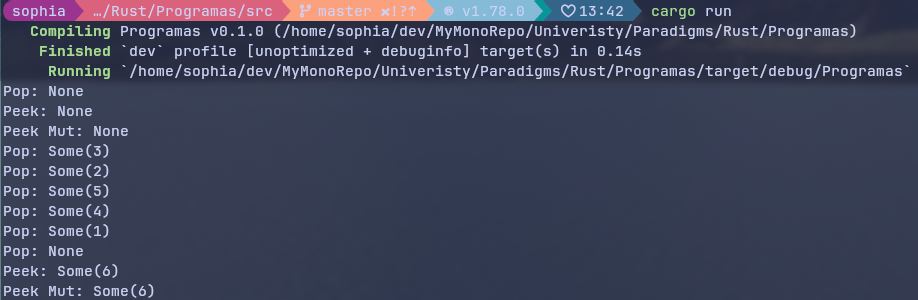
\includegraphics[scale=0.4]{ListRun}

Fonte: https://rust-unofficial.github.io/too-many-lists/

%%%--------------------------------------------------------------------
\section{Quick Sort}
%%%--------------------------------------------------------------------
  Organiza um vetor de n\'{u}meros usando o m\'{e}todo de parti\c{c}\~{a}o conhecido como quicksort

\begin{lstlisting}[language=rust]
quick.rs
extern crate std as core;

use core::cmp::Ordering;

fn quicksort_helper<T, F>
  (arr: &mut [T], left: isize, right: isize, compare: &F)
where F: Fn(&T, &T) -> Ordering {
    if right <= left {
        return
    }

    let mut i: isize = left - 1;
    let mut j: isize = right;
    let mut p: isize = i;
    let mut q: isize = j;

    unsafe {
        let v: *mut T = &mut arr[right as usize];
        loop {
            i += 1;
            while compare(&arr[i as usize], &*v) == Ordering::Less {
                i += 1
            }
            j -= 1;
            while compare(&*v, &arr[j as usize]) == Ordering::Less {
                if j == left {
                    break
                }
                j -= 1;
            }
            if i >= j {
                break
            }
            arr.swap(i as usize, j as usize);
            if compare(&arr[i as usize], &*v) == Ordering::Equal {
                p += 1;
                arr.swap(p as usize, i as usize)
            }
            if compare(&*v, &arr[j as usize]) == Ordering::Equal {
                q -= 1;
                arr.swap(j as usize, q as usize)
            }
        }
    }

    arr.swap(i as usize, right as usize);
    j = i - 1;
    i += 1;
    let mut k: isize = left;
    while k < p {
        arr.swap(k as usize, j as usize);
        k += 1;
        j -= 1;
        assert!(k < arr.len() as isize);
    }
    k = right - 1;
    while k > q {
        arr.swap(i as usize, k as usize);
        k -= 1;
        i += 1;
        assert!(k != 0);
    }

    quicksort_helper(arr, left, j, compare);
    quicksort_helper(arr, i, right, compare);
}
\end{lstlisting}

\begin{lstlisting}[language=rust]
pub fn quicksort_by<T, F>
  (arr: &mut [T], compare: F) where F: Fn(&T, &T) -> Ordering {
    if arr.len() <= 1 {
        return
    }

    let len = arr.len();
    quicksort_helper(arr, 0, (len - 1) as isize, &compare);
}

/// An in-place quicksort for ordered items.
#[inline]
pub fn quicksort<T>(arr: &mut [T]) where T: Ord {
    quicksort_by(arr, |a, b| a.cmp(b))
}
\end{lstlisting}
\newpage
\begin{lstlisting}[language=rust]
fn main() {
    let mut rng = rand::thread_rng();
    let len: usize = rng.gen();
    let mut v: Vec<isize> = rng.gen_iter::<isize>().take((len % 32) + 1).collect();
    for i in 0 .. v.len() - 1 {
        v[i] = v[i] % 1000;
    }
    quicksort(&mut v);
    println!("Unsorted:");
    for i in 0 .. v.len() - 1 {
        println!("{}", v[i])
    }
     println!("Sorted:");
    for i in 0 .. v.len() - 1 {
        println!("{}", v[i])
    }
}
\end{lstlisting}

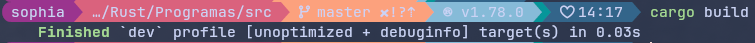
\includegraphics[scale=0.4]{QuickBuild}
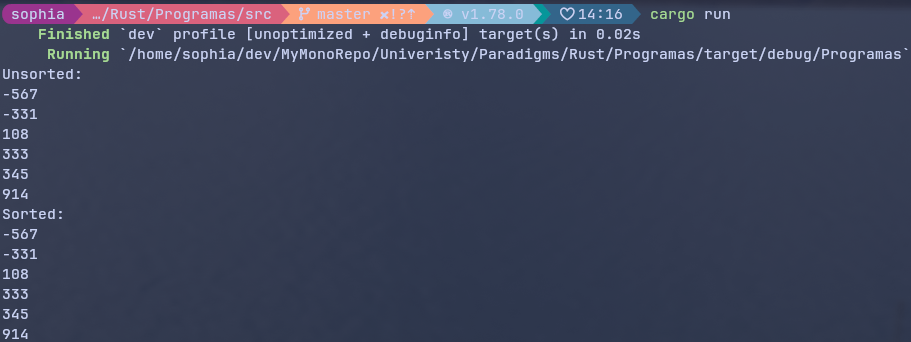
\includegraphics[scale=0.4]{QuickRun}

Fonte: http://www.cs.princeton.edu/~rs/talks/QuicksortIsOptimal.pdf

\pagebreak
\newpage
%%%--------------------------------------------------------------------
\section{IsPrime}
%%%--------------------------------------------------------------------
Verifica se um numero \'{e} primo

\begin{lstlisting}[language=rust]
prime.rs
fn main() {
    let num = 17;
    if is_prime(num) {
        println!("{} is prime", num);
    } else {
        println!("{} is not prime", num);
    }
}

fn is_prime(n: u32) -> bool {
    if n <= 1 {
        return false;
    }
    for i in 2..=n / 2 {
        if n % i == 0 {
            return false;
        }
    }
    true
}
\end{lstlisting}

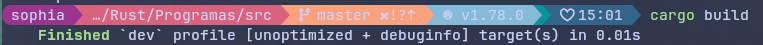
\includegraphics[scale=0.4]{PrimeBuild}
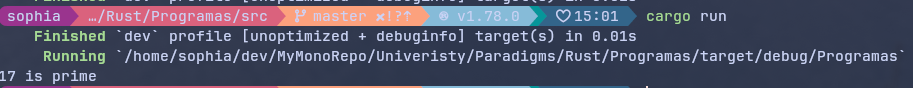
\includegraphics[scale=0.4]{PrimeRun}

Este c\'{o}digo \'{e} original deste livro
\pagebreak
\newpage

%%%--------------------------------------------------------------------
\section{Binary Search}
%%%--------------------------------------------------------------------
Verifica se um numero \'{e} primo

\begin{lstlisting}[language=rust]
binary.rs

fn main() {
    let arr = [1, 3, 5, 7, 9, 11, 13, 15, 17, 19];
    let target = 1;

    if let Some(index) = binary_search(&arr, target) {
        println!("Element {} found at index {}", target, index);
    } else {
        println!("Element {} not found in the array", target);
    }
}

fn binary_search(arr: &[i32], target: i32) -> Option<usize> {
    let mut left = 0;
    let mut right = arr.len() - 1;

    while left <= right {
        let mid = left + (right - left) / 2;
        if arr[mid] == target {
            return Some(mid);
        } else if arr[mid] < target {
            left = mid + 1;
        } else {
            right = mid - 1;
        }
    }
    None
}
\end{lstlisting}

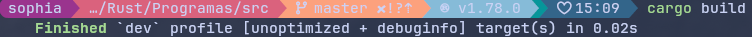
\includegraphics[scale=0.4]{BinaryBuild}
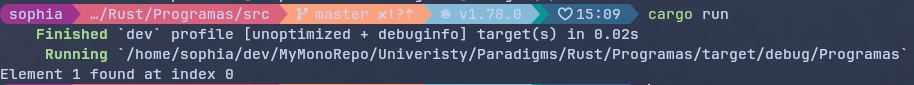
\includegraphics[scale=0.4]{BinaryRun}

Este c\'{o}digo \'{e} original deste livro

% Prof. Dr. Ausberto S. Castro Vera
% UENF - CCT - LCMAT - Curso de Ci\^{e}ncia da Computa\c{c}\~{a}o
% Campos, RJ,  2023
% Disciplina: Paradigmas de Linguagens de Programa\c{c}\~{a}o
% Aluno:



\chapterimage{ScalaH} % Chapter heading image ==>  Trocar este arquivo por outro 1200x468
\chapter{Ferramentas}

Aqui exploraremos as ferramentas que permitem que a promação em Rust seja facil e rapido, e disponibilize para nos o que precisamos para achar erros nos nossos codigos compila-los e publicalos

    \section{RustUp}

    Download: https://rustup.rs/

    Rustup é uma ferrmenta que baixa configura e instala todo o ecossistema Rust para você sem que você tenha que se preocupar com sistema, versoes, etc.

    Atualmente se encontra na versão 1.27.1

    Para usar rustup basta que você apenas rode o seguinte comando no seu terminal:

    \begin{lstlisting}[language=rust]
      curl --proto '=https' --tlsv1.2 -sSf https://sh.rustup.rs | sh
    \end{lstlisting}


    \section{Cargo}

    Cargo é o package manager e project manager do Rust, isso significa que ele é responsavel por pegar as dependencias dos seus projetos e gerenciar seus projetos.

    Cargo é instalado pelo programa Rustup.

    Para usalo basta apenas iniciar um projeto com "cargo init" isso criara uma pasta com o arquivo "cargo.toml" e uma pasta src com um arquivo "main.rs", no arquivo cargo.toml basta apenas escrever os nomes das dependencias que voce deseja incluir em seu projeto. para testar o seu projeto use "Cargo run", para criar um novo modulo basta usar "Cargo new" e para compilar e exportar o seu projeto basta usar "Cargo build".





% Prof. Dr. Ausberto S. Castro Vera
% UENF - CCT - LCMAT - Curso de Ci\^{e}ncia da Computa\c{c}\~{a}o
% Campos, RJ,  2023
% Disciplina: Paradigmas de Linguagens de Programa\c{c}\~{a}o
% Aluno: Eric Hoffmann Fernandes Braga


\chapterimage{ScalaH} % Chapter heading image
\chapter{Considera\c{c}\~{o}es Finais}
O trabalho que foi desenvolvido em forma resumida explica as origens e funcionamento da linguagem Rust, dando ao leitor conhecimento suficiente da linguagem e seu ecossistema para que continue sozinho e desenvolva ìncriveis aplicações.

\par
Os livros usados de referência foram:
\par
https://doc.rust-lang.org/stable/book/
\par
https://doc.rust-lang.org/stable/rust-by-example/











\chapterimage{Bibliografia.png}
\bibliographystyle{alpha}
\bibliography{Rust}
\addcontentsline{toc}{chapter}{\textcolor{ocre}{Bibliografia}}
%----------------------------------------------------------------------------------------
%	INDEX
%----------------------------------------------------------------------------------------

\cleardoublepage
\phantomsection
\setlength{\columnsep}{0.75cm}
\addcontentsline{toc}{chapter}{\textcolor{ocre}{Index}}
\printindex

%----------------------------------------------------------------------------------------

\end{document}

